\begin{sleekbox}[palTeal]{Problem #1}
    \begin{question}\leavevmode\par\medskip
        \anglevector{1,3,5}+\anglevector{7,-2,-4}
    \end{question}\leavevmode\par\medskip
    
    \begin{solution}\leavevmode\par\medskip
        \anglevector{1+7,3-2,5-4} = \anglevector{8,1,1}
    \end{solution}
\end{sleekbox}

\begin{sleekbox}[palTeal]{Problem #2}
    \begin{question}\leavevmode\par\medskip
        \anglevector{1,3,5} - \anglevector{7,-2,-4}
    \end{question}\leavevmode\par\medskip
        
    \begin{solution}\leavevmode\par\medskip
        \anglevector{-6,5,9}
    \end{solution}
\end{sleekbox}

\begin{sleekbox}[palTeal]{Problem #3}
    \begin{question}\leavevmode\par\medskip
        6\anglevector{1,3,5}
    \end{question}\leavevmode\par\medskip
        \anglevector{6,18,30}
    \begin{solution}\leavevmode\par\medskip
        
    \end{solution}
\end{sleekbox}

\begin{sleekbox}[palTeal]{Problem #4}
    \begin{question}\leavevmode\par\medskip
        \anglevector{1,3,5} \cdot \anglevector{7,-2,-4}
    \end{question}\leavevmode\par\medskip

    \begin{solution}\leavevmode\par\medskip
        $7-6-20=-19$
    \end{solution}
\end{sleekbox}


\begin{sleekbox}[palTeal]{Problem #5}
    \begin{question}\leavevmode\par\medskip
        \norm{\anglevector{1,3,5}}
    \end{question}\leavevmode\par\medskip

    \begin{solution}\leavevmode\par\medskip
        \sqrt{1+9+25} = \sqrt{35}
    \end{solution}
\end{sleekbox}

\begin{sleekbox}[palTeal]{Problem #6}
    \begin{question}\leavevmode\par\medskip
        \norm{\anglevector{7,-2,-4}}
    \end{question}\leavevmode\par\medskip
    
    \begin{solution}\leavevmode\par\medskip
        \sqrt{49+4+16} = \sqrt{69}
    \end{solution}
\end{sleekbox}

\begin{sleekbox}[palTeal]{Problem #7}
    \begin{question}\leavevmode\par\medskip
        Find the angle between \anglevector{1,3,5} and \anglevector{7,-2,-4}.
    \end{question}\leavevmode\par\medskip

    \begin{solution}\leavevmode\par\medskip
        \[
        \anglevector{1,3,5} \cdot \anglevector{7,-2,-4} = \norm{\anglevector{1,3,5}}\norm{\anglevector{7,-2,-4}}\cos(\theta) \implies \frac{-19}{\sqrt{2415}} = \cos(\theta)
        \]
        \[
        \implies \theta =\cos^{-1}(\frac{-19}{\sqrt{2415}}) \approx 1^{\circ}\footnotemark
        \]
    \end{solution}\footnotetext{Rounded to the 5th decimal place.}
\end{sleekbox}

\begin{sleekbox}[palTeal]{Problem #8}
    \begin{question}\leavevmode\par\medskip
        Find the dot product of the vectors \anglevector{7,3,-1,4},\anglevector{5,9,2,5} \in \R^4 .
    \end{question}\leavevmode\par\medskip

    \begin{solution}\leavevmode\par\medskip
        \anglevector{7,3,-1,4} \cdot\anglevector{5,9,2,5} = 35 + 27 - 2 + 20 = 80
    \end{solution}
\end{sleekbox}

\begin{sleekbox}[palTeal]{Problem #9}
    \begin{question}\leavevmode\par\medskip
        Given two vectors whose dot product is zero. What can you say about the
        vectors? Give an example of two vectors with this property.
    \end{question}\leavevmode\par\medskip

    \begin{solution}\leavevmode\par\medskip
        \[
        \forall \, \Vec{u},\Vec{v}\in V_n \subset \R^n , \text{where } \Vec{u} \cdot \Vec{v} = 0 \implies \cos(\theta) = 0 \implies \theta = 0 + 2\pi c, \text{ for } c \in \mathbb{Z}
        \]
        Thus both vectors must be orthogonal to one another. An example of this property are the unit vectors where the dot product for any 2 unique standard vectors $(\hat{i},\hat{j},\hat{k},\dots)$ is zero. Thus all of the standard unit vectors are orthogonal to one another.
    \end{solution}
\end{sleekbox}

\begin{sleekbox}[palTeal]{Problem #10}
    \begin{question}\leavevmode\par\medskip
        \begin{parts}
            \item Find a vector orthogonal to the vectors \anglevector{2,17,5}, and \anglevector{-1,-4,-7}.
            \item Show (by calculations on Mathematica) that these vectors are orthogonal.
            \item Graph the three vectors.
        \end{parts}
        
    \end{question}\leavevmode\par\medskip

    \begin{solution}\leavevmode\par\medskip 
        \begin{parts}
            \item  \[
            \anglevector{2,17,5} \times \anglevector{-1,-4,-7} = \begin{vmatrix} \hat{i} & \hat{j} & \hat{k} \\ 2 & 17 & 5 \\ -1 & -4 & -7 \end{vmatrix} = \begin{vmatrix} 17 & 5 \\ -4 & -7 \end{vmatrix} \hat{i} - \begin{vmatrix} 2 & 5 \\ -1 & -7 \end{vmatrix} \hat{j} = \begin{vmatrix} 2 & 17 \\ -1 & -4\end{vmatrix} \hat{k}
            \]
    
            \[
            = \anglevector{-99,9,9}
            \]

            \item \[
                \anglevector{2,17,5} \cdot \anglevector{-99,9,9} = 0 \wedge \anglevector{-1,-4,-17} \cdot \anglevector{-99,9,9} = 0
            \]
        \end{parts}
       
        
    \end{solution}
\end{sleekbox}

\begin{sleekbox}[palTeal]{Problem #11}
    \begin{question}\leavevmode\par\medskip
    Sketch the surface by hand (if possible) and also using Mathematica (plot3D):
    \begin{parts}
        \item $f(x,y) = 1-x^2-y^2$
        \item $f(x,y)=\sqrt{1-x^2 -z^2}$
    \end{parts}
        
    \end{question}\leavevmode\par\medskip
       
    \begin{solution}\leavevmode\par\medskip
         \begin{figure}[H]
            \centering
            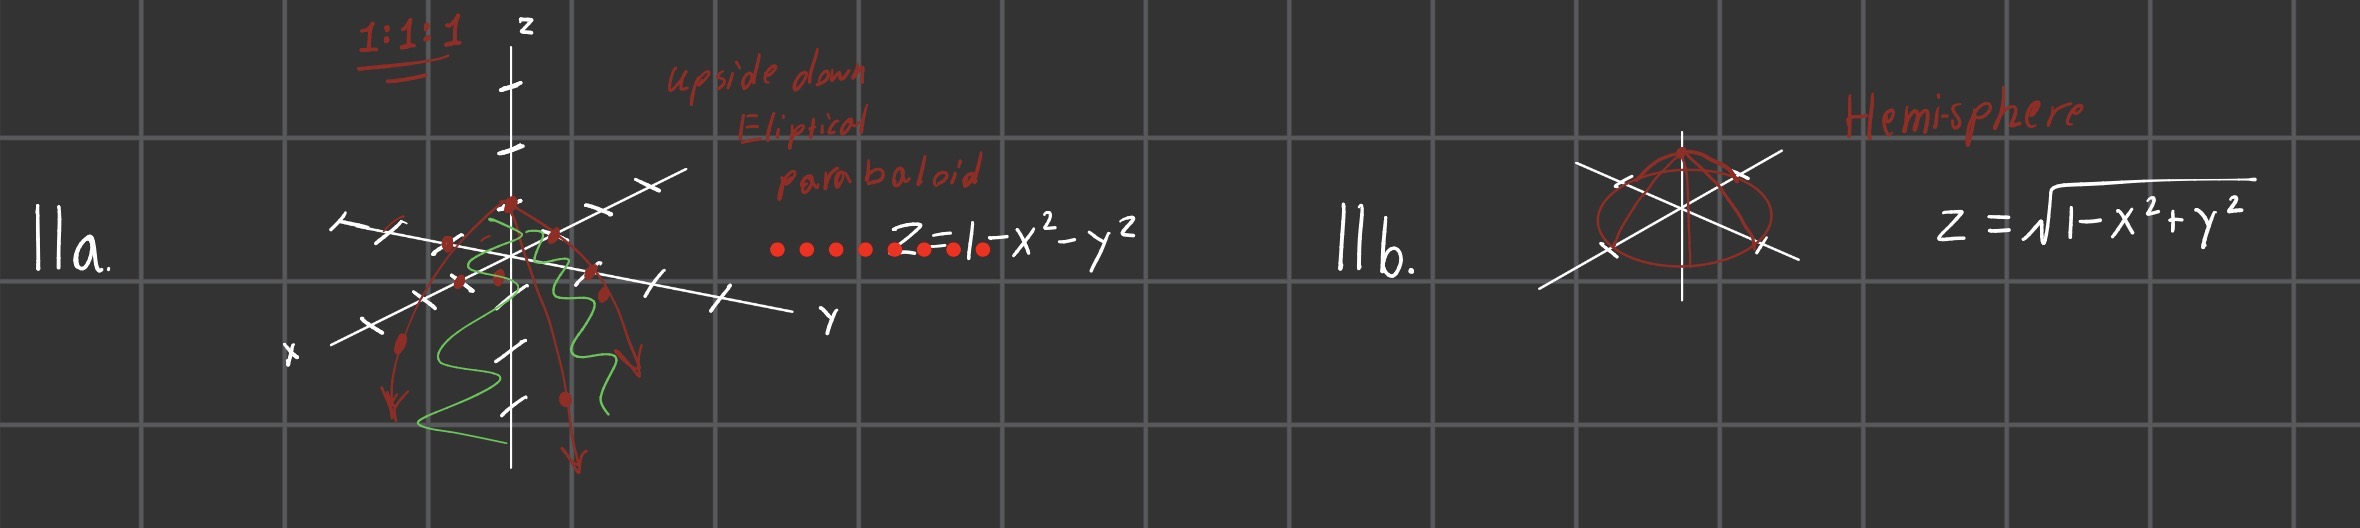
\includegraphics[width=0.75\linewidth]{Unit 13//Lab 1/IMG_2660.jpeg}
            \label{fig:placeholder}
        \end{figure}
    \end{solution}

\end{sleekbox}